\documentclass[UTF8,12pt,a4paper]{ctexart}
\usepackage[left=31.75mm,right=31.75mm,top=25.4mm,bottom=25.4mm]{geometry}
\setmainfont{Times New Roman}
\setCJKmainfont[AutoFakeBold=2]{SimSun}
\usepackage{graphicx,float,longtable,booktabs,array,amsmath,hyperref}
\hypersetup{hidelinks,pdfauthor={},pdftitle={基于FPGA的心电边缘分析系统}}
\newcolumntype{L}[1]{>{\raggedright\arraybackslash}p{#1}}
\setcounter{secnumdepth}{0}
\setlength{\parindent}{2em}
\graphicspath{{figures/}}
% TeX是内容主源。最终PDF由转换后的Word直接导出，以同一排版核对。
% 2026-11-03按双模型硬件加速修订；预算与模板限字以word_counts.json实际统计。
\begin{document}
\begin{center}
{\zihao{-2}\bfseries 基于FPGA的心电边缘分析系统}\par
技术文档
\end{center}

\section{摘要}
% COUNT_BEGIN:abstract:800
本作品构建基于Zynq-7020的心电边缘分析系统。ADS1292R与STM32经JDY18将数据送至电脑，电脑解包、换算、保存并通过USB串口送入Zynq。ARM执行高通、QRS检测、切拍、形态及RR历史特征，PL分别实现HGB树分类和H27一维CNN全网络，网页显示逐拍类别、概率及实测性能。HGB以三类并行树遍历实现Q40计算；CNN采用四输出通道并行、流水线及分区片上存储，保持FP32计算口径。同一5148点记录的三次CNN整段测量，每次12个有效心拍，ARM网络平均8272.33微秒/拍，PL含传输2763.25微秒/拍，累计加速2.994倍；同镜像HGB含传输加速1.914倍。100MHz双模型设计占LUT16.86\%、BRAM71.79\%、DSP17.27\%。500Hz开发回归QRS灵敏度99.8731\%、阳性预测值99.8453\%。倍率只对应模型计算调用，不代表整机或临床效果。

% COUNT_END:abstract
% RESERVE:abstract_final:0:摘要
\begin{figure}[H]\centering
\includegraphics[width=\linewidth,height=0.6cm]{blank.png}\end{figure}

\section{第一部分 作品概述}
\subsection{1.1 功能与特性}
% COUNT_BEGIN:functions:400
系统支持34字节帧接收、CSV回放、原始记录和网页显示。检测路径返回R峰、RR及心率；用户可选HGB整段分类、CNN整段或逐拍分类，查看类别、概率及ARM/PL计时。两种模型独立执行，结果保留来源、执行位置及有效状态，停止后保存历史。

% COUNT_END:functions
\subsection{1.2 应用领域}
% COUNT_BEGIN:applications:400
作品用于生物电处理与FPGA协同计算原型研究，以公开数据评价识别质量、实测CSV核对通路，不承担医疗诊断功能。
% COUNT_END:applications
\subsection{1.3 主要技术特点}
% COUNT_BEGIN:technical:400
以统一单位、源样本时轴和会话状态贯通采集与结果。ARM负责控制和特征，PL按模型结构采用并行树或卷积加速；固定权重及相同精度参考逐拍核对，计时分离计算和传输。CNN使用有界缓存持续处理，显示滤波不改变模型输入。

% COUNT_END:technical
\subsection{1.4 主要性能指标}
% COUNT_BEGIN:indicators:200
\begin{longtable}{L{0.33\linewidth}L{0.59\linewidth}}
\toprule 指标 & 实测结果及口径 \\ \midrule
500Hz QRS & Se99.8731\%；PPV99.8453\% \\
模型调用加速 & CNN2.994倍；HGB1.914倍 \\
双模型PL & 100MHz；8972 LUT；100.5 BRAM；38 DSP \\
\bottomrule
\end{longtable}

% COUNT_END:indicators
\subsection{1.5 主要创新点}
% COUNT_BEGIN:innovation:200
（1）按模型结构分别实现并行树与FP32卷积，形成同一平台上的两条硬件加速路径。（2）统一源样本位置、单位及状态，使结果能对应原始波形。（3）用同输入、同精度ARM参考逐拍核验PL，分别测量计算与传输。以上为工程实现特点，公开算法来源随工程保留。

% COUNT_END:innovation
\subsection{1.6 设计流程}
% COUNT_BEGIN:designflow:200
冻结输入与评价，逐级验证C、ARM、PL及网页，保留各阶段证据。
% COUNT_END:designflow
% RESERVE:overview_final:0:作品概述
\begin{figure}[H]\centering
\includegraphics[width=\linewidth,height=0.8cm]{blank.png}\end{figure}

\section{第二部分 系统组成及功能说明}
\subsection{2.1 整体介绍}
采集模块经无线发送双通道数据，电脑分别连接USB接收器和Zynq USB\_UART。板端提供检测、整段分类及CNN逐拍分类；事件均带源位置，网页区分模型与执行位置。
\begin{figure}[H]\centering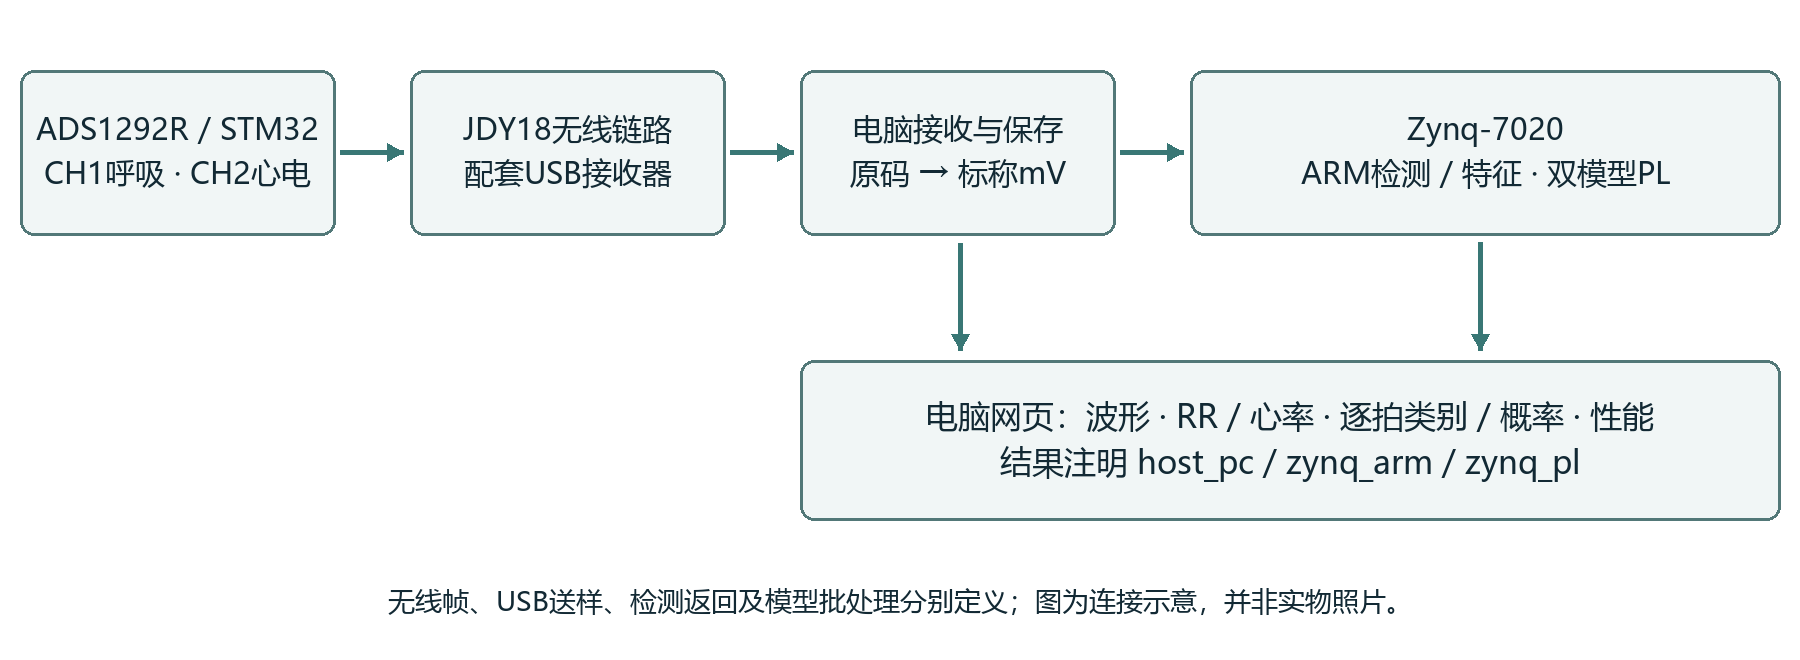
\includegraphics[width=\linewidth]{system.png}\caption{系统连接与数据方向示意，非实物照片}\end{figure}

\subsection{2.2 硬件系统介绍}
平台为领航者V2与Zynq-7020，采用Vivado/Vitis 2026.1、裸机与XSim[1,2]。DDR存放输入及工作区，QSPI启动固化镜像，JTAG运行双模型镜像。镜像身份、下载和冷启动分别记录。
\begin{figure}[H]\centering
\includegraphics[width=\linewidth,height=0.6cm]{blank.png}\end{figure}

采用现成开发板和ADS1292R模块。STM32发送34字节帧：AA BB帧头加4组双通道采样，每通道4字节大端容器表示偏置24位码；CH1呼吸、CH2心电。

偏置码减8388608得到有符号值。模块方确认参考电压2.42V、增益6，报告按标称参数换算。项目标称换算为
\[
v_{\mathrm{mV}}=C_{\mathrm{signed}}\frac{2420}{6\times8388607}.
\]
手册理想分母为$2^{23}$[3]，相对差约0.000012\%；标称换算不等同仪器标定。算法按4096单位/mV转换int16，半值远离零舍入并饱和，同时保留原码和mV。

PL保留QRS/HGB外设，增加CNN AXI-Lite外设0x43C20000；模型输入和结果经寄存器交换，沿用既有PS7、DDR与MIO配置。

\subsection{2.3 软件系统介绍}
\subsubsection{2.3.1 分层与通信}
网页采用React/TypeScript与FastAPI，负责记录、回放及显示，Tk备用。ARM完成检测、特征、PL调用与softmax；网页保存执行位置和计时。
\begin{figure}[H]\centering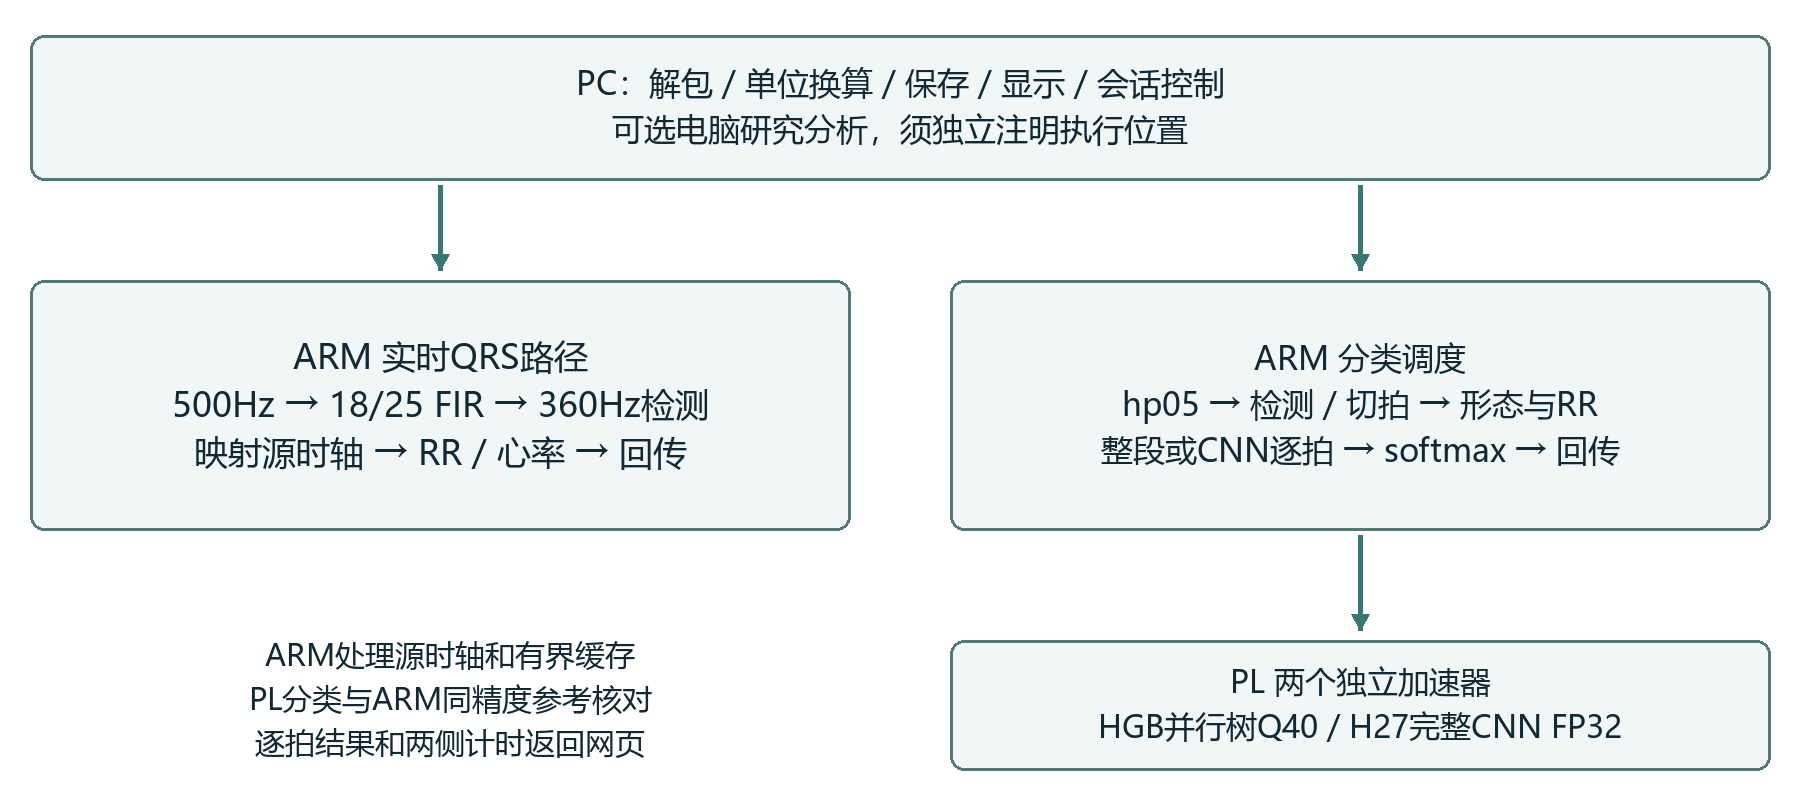
\includegraphics[width=\linewidth]{partition.png}\caption{ARM与PL分工及两条业务路径}\end{figure}

厂商34字节协议只用于模块到电脑；ECG-IN-1用于电脑向实时检测路径送样，含配置、序号、CRC及确认；ECG-UART-1返回事件与状态。HGB、CNN整段及CNN-STREAM-1分别约束模型输入和返回，避免三类与四类混用。USB\_UART采用115200、8N1、无流控，能够双向通信，协议仍按确认和背压限制发送。

样本从0编号，以源位置和采样率计时；缺口、重连或增益变化时重置会话并保存现场。厂商无每点设备序号，电脑编号不证明无线零丢样。

\subsubsection{2.3.2 滤波、检测及切拍}
绘图归一化至$[-1,1]$，不改保存数据。呼吸显示采用0.05Hz高通及0.8Hz二阶低通；显示波形与生理指标分开，显示滤波不替代模型输入。

实时路径经1001系数18/25 FIR将500Hz转为360Hz，送入冻结检测器并映射回源时轴，按检测事件切拍。核心参考WFDB与NeuroKit梯度思路，保留来源、改动和许可[6,7]。

模型路径默认接收未额外数字滤波的500Hz单导联mV，执行指定0.5Hz因果高通：
\[
a=\frac{500}{500+2\pi\times0.5},\quad y_0=0,\quad
y_n=a(y_{n-1}+x_n-x_{n-1}).
\]
使用float64并延续分块状态。模型重定位R峰，取前178点及从R起267点，转换为144Hz、128点波形。HGB形成192项特征，后继RR最多等待2.5秒；CNN仅用当前窗及因果历史，在窗口就绪后分类。首RR或窗口不足输出UNCLASSIFIED。

\subsubsection{2.3.3 两种模型与软硬件分工}
HGB固定v92/fold0，输出N/S/VF，VF合并V/E/F；CNN固定H27/fold0，输出N/S/V/F。N不是健康判定，VF不是心室颤动。fold0用于固定联调，不按验证分数挑选；两模型不是投票集成。

H27包含25,476个参数，输入为128点波形与差分、RR分支、122项形态/已完成背景和最近8个RR，分类头输入269维。ARM准备波形及外部特征，PL执行卷积、三残差块、最大池化、RR分支和全连接，ARM执行softmax。FP32与树模型Q40分别核验，不将其称为INT8。

CNN逐拍路径采用4096点环形缓存、32项事件队列、8个已完成背景和有界RR历史，跨传输块保留状态。窗口就绪后返回逐拍结果，避免反复重算已处理前缀；中止不强补尾窗。

\subsubsection{2.3.4 硬件加速实现}
HGB将64轮、三类共192棵树按类别并行遍历。float32输入的阈值转换保持原double分支判断，叶值和基线为64位Q40，按原顺序累加；ARM同Q40参考核对分数，随后计算概率。树节点和参数映射片上存储，减少通用指令调度开销。

CNN采用HLS实现FP32运算。卷积每组展开4个输出通道，4路权重与累加器独立分区；输入特征被复用，时间位置循环流水化，空间交错累加避免同一地址的连续相关。局部乘法映射DSP，保留每一路原点积累加顺序，禁止融合乘加改变舍入；残差、ReLU、池化及全连接与参考逐层衔接。
\[
z_{o,t}=\sum_i\sum_k x_{i,t+k-p}w_{o,i,k}.
\]
4个输出通道并行，并不表示整个网络所有层同时运行。AXI-Lite完成261项输入写入、启动、完成轮询与4项logit读取。软件将寄存器调用与计算等待分别计时，以展示并行收益及接口开销；100MHz时序由布局布线报告核对。
% RESERVE:system_final:0:系统与功能

\subsection{2.4 复现方法}
按教程建立独立环境，依次检查仓库、模型、主机C、仿真及实现；从固定权重在新目录重建。核对bit/XSA/ELF/FSBL身份后下载，以报文、样本数及分类结果验收。

\section{第三部分 完成情况及性能参数}
\subsection{3.1 实物与界面}
当前采用现成模块与开发板，自研内容为逻辑、ARM应用和电脑软件。下列图位用于放置与演示版本一致的实物、连接及网页截图。
\begin{longtable}{L{0.46\linewidth}L{0.46\linewidth}}
系统正面全局 & 系统斜45度全局 \\

\includegraphics[width=5.9cm,height=2.2cm]{blank.png} & 
\includegraphics[width=5.9cm,height=2.2cm]{blank.png} \\
电路与关键连接 & 软件界面与板端结果 \\

\includegraphics[width=5.9cm,height=2.2cm]{blank.png} & 
\includegraphics[width=5.9cm,height=2.2cm]{blank.png} \\
\end{longtable}

\subsection{3.2 评价方法与QRS结果}
以专家标注计TP/FN/FP及定位、RR误差，分类报告逐类指标和混淆矩阵，专家切拍与端到端评价分开。同人不跨集合，201/202按同人处理；42条MIT-BIH均已查看，仅为开发回归[4,9]；患者隔离仍不能消除反复选型的偏差[8]。
\begin{longtable}{L{0.48\linewidth}L{0.44\linewidth}}
\toprule 500Hz配对路径指标 & 既有结果 \\ \midrule
TP / FN / FP & 96787 / 123 / 150 \\
灵敏度 / 阳性预测值 & 99.8731\% / 99.8453\% \\
定位 / RR平均绝对误差 & 2.8097ms / 2.8741ms \\
逐记录达到原门槛 & 41/42；105号FP66、FN10 \\
\bottomrule
\end{longtable}
500Hz与360Hz配对阶段等效；105号噪声误检及原门槛失败保留。实测波形无逐拍专家标注，仅核对通路和数值。

\subsection{3.3 分类质量}
INCART按患者三折留出[5]，外折使用对应模型计分；部署统一fold0不改变评价划分。封存患者8、10、22、23、31、32保持隔离。表中均为开发评价，端到端漏检与额外预测计入，专家切拍另列证据。
\begin{longtable}{L{0.28\linewidth}L{0.30\linewidth}L{0.34\linewidth}}
\toprule 模型 & S精确率/召回率 & 汇总指标 \\ \midrule
HGB三类hp05 & 53.71\% / 81.63\% & macro-F1 86.12\% \\
H27四类 & 50.36\% / 83.69\% & macro-F1 69.10\% \\
H27的F类 & 30.00\% / 16.77\% & F1 21.51\% \\
\bottomrule
\end{longtable}
H27总体参考拍准确率97.70\%，但类别不均衡使总体值不能代替S/F评价。HGB的VF与CNN的V、F语义不同，不直接比较宏指标高低；移植一致性也不提高识别质量。

\subsection{3.4 同条件硬件加速实验}
比较在同一Zynq-7020上进行，各模型分别使用相同输入、权重和精度。ARM计时器约333.33MHz，PL为100MHz。5148点ADS记录产生13个事件、12个有效心拍；表中CNN取独立回放及两次网页回放共3轮、36次有效网络调用，将累计ARM时间除以累计PL调用时间计算倍率。HGB为同镜像、同记录的网页回放12拍。
\[
S_{\mathrm{call}}=\frac{\sum_jT_{\mathrm{ARM},j}}{\sum_jT_{\mathrm{PLcall},j}}.
\]
\begin{longtable}{L{0.20\linewidth}L{0.24\linewidth}L{0.27\linewidth}L{0.21\linewidth}}
\toprule 模型/精度 & ARM微秒/拍 & PL调用微秒/拍 & 加速倍率 \\ \midrule
H27 FP32 & 8272.33 & 2763.25 & 2.994 \\
HGB Q40 & 94.83 & 49.54 & 1.914 \\
\bottomrule
\end{longtable}
CNN三轮调用倍率为2.9927—2.9947；PL计算等待平均2705.06微秒/拍，由ARM轮询计时，含轮询开销。HGB硬件周期计数对应纯核7.625微秒/拍，纯核约12.44倍；它不与CNN轮询时间混为同一种测量。上述均排除QRS、特征、softmax、USB串口及网页，不能称整机三倍或十二倍。

CNN的12组黄金向量经HLS C与RTL联合仿真，最大logit差约$2.861\times10^{-6}$；RTL延迟270490—270492周期。板上按$2\times10^{-4}+2\times10^{-5}|r|$容差及相同argmax核对，5148点与30000点回放的位置、状态、类别一致，概率最大差分别约$8.74\times10^{-10}$与$1.20\times10^{-6}$；ARM/PL不一致数为0。HGB既有492组仿真和160组特征实板对照也保留。

\subsection{3.5 资源占用与持续处理}
\begin{longtable}{L{0.32\linewidth}L{0.30\linewidth}L{0.30\linewidth}}
\toprule 资源 & 已用/可用 & 占比 \\ \midrule
LUT & 8972 / 53200 & 16.86\% \\
FF & 8866 / 106400 & 8.33\% \\
BRAM tile & 100.5 / 140 & 71.79\% \\
DSP & 38 / 220 & 17.27\% \\
\bottomrule
\end{longtable}
数据来自双模型全设计布局布线，包含QRS、HGB、CNN及互连，非CNN独占资源。100MHz下WNS0.270ns、WHS0.036ns。较高BRAM占用来自权重及中间存储，4通道并行在计算速度、存储端口和时序之间取舍；资源余量不等于运行闲置，也不以占满资源为优化目标。

500Hz节拍的60秒合成回放共30000点、73事件、72有效拍，CNN网络ARM累计593.855ms，PL含传输累计198.960ms，比值2.985。32768点回放得到79事件、78有效拍，验证环形缓存跨整段上限工作。真实记录最大算法等待618ms，合成608ms，属于R峰至所需输入就绪时间，不被网络加速倍率直接缩短。网页CNN逐拍、HGB整段及CNN整段可轮换运行，完整轮之间无须复位，主动停止保留已得事件。

资源占用与运行负载分别统计；点数、有效拍数及耗时须对应同轮输入，不以CSV行数或绘图刷新率推导PL忙碌占比。视频引用对应轮次原始记录。
% RESERVE:results_final:180:完成情况与性能
\begin{longtable}{L{0.50\linewidth}L{0.42\linewidth}}
\toprule 补充测量栏 & 实测记录 \\ \midrule
视频对应输入、轮数和计时摘要 & \\
完整链路耗时、内存峰值和功耗 & \\
实物照片及界面截图编号 & \\
\bottomrule
\end{longtable}

\section{第四部分 总结}
\subsection{4.1 可扩展之处}
% COUNT_BEGIN:extensions:300
系统形成采集格式接收、ARM检测与特征、双模型PL推理及网页显示的闭环。树模型展示分支遍历并行，CNN展示卷积并行与流水线；持续CNN通过有界状态衔接逐拍输入。本版采用FP32与Q40保持参考口径；INT8量化按独立精度和资源实验评价。更大并行度需同时考虑BRAM端口、DSP和时序，真实无线长时及带专家标注的评价应采用各自独立实验，不由数字回放推导。

% COUNT_END:extensions

\subsection{4.2 心得体会与AI协作}
% COUNT_BEGIN:reflection:1000
协作中由人确认目标、硬件条件及采纳依据，AI负责查资料、写实现与组织回归。原码、物理单位、显示归一化和识别质量分别验证；程序写入成功也不能替代冷启动与负载检查。

\subsubsection{原始提示、对应回答与纠错摘录}
2026年10月25日，用户：“你这个交接写的有问题，是别人用这个工程，不是我。”AI：“我会把交接改成面向接手者：说明他拿到工程后怎么启动、需要准备什么、哪些结果可以复用，去掉依赖你这台电脑和本次聊天的表述。”

2026年10月26日，用户：“原始数据是经过ADC放大的，不是真实电压值”。AI：“上次说‘直接接收能用’省略了换算这一步，容易让你误解。”后续核查区分配套10字节源码与实际34字节固件，只认可有来源的标称参数，不声称已读取实机寄存器或完成标定。

以上节选自封存会话S01的M0016—M0017、M0026—M0028，省略上下文及本机路径，仅调整双层引号。原文时间、源行和SHA索引保存在本地写作附件。

\subsubsection{人工采纳依据与个人补充}
用户要求交接面向实际接手者，并纠正把原码直接理解为电压的表述，因此采用参数回查、单位合同和分级验收。文件字节受Git换行转换影响后，采用实际克隆核对；启动头误拒后，先查校验器的位宽和符号，不盲目擦写。没有采纳降低QRS门槛、删困难段或将未知拍填N的做法。

上述经验提炼为artifact-check、trace-check和download-diagnose。前两项抽出文件哈希与同一时轴比对脚本，独立副本合计12项行为测试通过；第三项区分编程、校验与启动。脚本通过不等于板卡验证，缺依赖的结构检查不算赛事认证。这些是已有记录支持的取舍，不代写未记录的个人体验。
% COUNT_END:reflection
% RESERVE:collaboration_final:0:总结与协作

\section{第五部分 参考文献}
\begin{enumerate}
\setlength{\itemsep}{0pt}
\item 全国大学生嵌入式芯片与系统设计竞赛. FPGA创新设计赛道选题指南 AMD[S]. 2026: 自主选题3.3.3—3.3.5.
\item AMD. Vitis嵌入式软件开发用户指南 UG1400[M]. 2026.1版, 2026.
\item Texas Instruments. ADS1291 ADS1292 ADS1292R 数据手册[Z]. 项目所附版本, 8.3.4及8.3.8节.
\item Moody G, Mark R. MIT-BIH Arrhythmia Database, version 1.0.0[DB/OL]. PhysioNet, 2005. DOI:10.13026/C2F305.
\item Yakushenko E. St Petersburg INCART 12-lead Arrhythmia Database, version 1.0.0[DB/OL]. PhysioNet, 2008. DOI:10.13026/C2V88N.
\item MIT-LCP. WFDB-Python qrs.py, version 4.3.1[CP/OL]. GitHub[2026-11-02]. 固定版本源码与MIT许可.
\item Makowski D, Pham T, Lau Z J, et al. NeuroKit2: A Python toolbox for neurophysiological signal processing[J]. Behavior Research Methods, 2021, 53(4):1689--1696. DOI:10.3758/s13428-020-01516-y.
\item Cawley G C, Talbot N L C. On Over-fitting in Model Selection and Subsequent Selection Bias in Performance Evaluation[J]. Journal of Machine Learning Research, 2010, 11(70):2079--2107.
\item Pollard T, Moody B E, Lehman L, et al. PhysioNet as a global platform for biomedical research[J]. Nature Health, 2026. DOI:10.1038/s44360-026-00096-z.
\end{enumerate}
\end{document}
